\qrchapter{https://forgottenpillar.com/rsc/en-fp-chapter1}{The Foundation of Our Faith}


\qrchapter{https://forgottenpillar.com/rsc/es-fp-chapter1}{El Fundamento de Nuestra Fe}


\egw{\textbf{The Lord will put new, vital force into His work} as human agencies obey the command to go forth and proclaim the truth. \textbf{He who declared that His truth would shine forever will proclaim this truth through faithful messengers, who will give the trumpet a certain sound}. \textbf{The truth will be criticized, scorned, and derided; but the \underline{closer} it is examined and tested, \underline{the brighter it will shine}}.}[SpTB02 51.1; 1904][https://egwwritings.org/read?panels=p417.260]


\egw{\textbf{El Señor pondrá nueva fuerza vital en su obra} a medida que los instrumentos humanos obedezcan la orden de avanzar y proclamar la verdad. \textbf{El que declaró que su verdad brillaría para siempre, proclamará esa verdad mediante mensajeros fieles, que darán a la trompeta un sonido certero}. \textbf{La verdad será criticada, desdeñada y ridiculizada; pero \underline{mientras más cerca} se la examine y se la pruebe, \underline{más brillará}}.}[SpTB02 51.1; 1904][https://egwwritings.org/read?panels=p417.260]


\egwnogap{\textbf{As a people, we are to \underline{stand firm on the platform of eternal truth} that has withstood test and trial. We are to \underline{hold to the sure pillars of our faith}. The \underline{principles of truth} that God has revealed to us \underline{are our only true foundation}. They have made us what we are. The lapse of time has not lessened their value. \underline{It is the constant effort of the enemy to remove these truths from their setting}, and to put in their place \underline{spurious theories}. He \underline{will bring in} everything that he possibly can to carry out his deceptive designs. But the Lord will raise up men of keen perception, who will give these truths their proper place in the plan of God.}}[SpTB02 51.2; 1904][https://egwwritings.org/read?panels=p417.261]


\egwnogap{\textbf{Como pueblo, hemos de \underline{mantenernos firmes en la plataforma de la verdad eterna} que ha resistido la prueba y el examen. Hemos de \underline{aferrarnos a las seguras columnas de nuestra fe}. Los \underline{principios de la verdad} que Dios nos ha revelado \underline{son nuestro único fundamento verdadero}. Nos han hecho lo que somos. El tiempo transcurrido no ha disminuido su valor. \underline{El enemigo se esfuerza constantemente por sacar esas verdades de su marco}, y poner en su lugar \underline{teorías espurias}. Él \underline{introducirá} todo lo que pueda para llevar a cabo sus designios engañosos. Pero el Señor hará surgir a hombres de percepción aguda, que darán a esas verdades su debido lugar en el plan de Dios.}}[SpTB02 51.2; 1904][https://egwwritings.org/read?panels=p417.261]


\egwnogap{\textbf{I have been instructed by the heavenly messenger that some of the reasoning in the book, ‘Living Temple,’ is unsound and that \underline{this reasoning would lead astray} the minds of those who are not thoroughly established on \underline{the foundation principles} of present truth. It introduces that which is naught but speculation in \underline{regard to the personality of God and where His presence is}}. No one on this earth has a right to speculate on this question. \textbf{The more fanciful theories are discussed, the less men will know of God and of the truth that sanctifies the soul}.}[SpTB02 51.3; 1904][https://egwwritings.org/read?panels=p417.262]


\egwnogap{\textbf{He sido instruida por el mensajero celestial de que parte del razonamiento del libro, ‘Living Temple,’ es malsano y que \underline{este razonamiento descarriaría} las mentes de aquellos que no están plenamente establecidos en \underline{los principios fundamentales} de la verdad presente. Introduce aquello que no es nada sino especulación en \underline{cuanto a la personalidad de Dios y dónde está su presencia}}. Nadie en esta tierra tiene derecho a especular sobre esta cuestión. \textbf{Mientras más se discutan las teorías fantásticas, los hombres sabrán menos de Dios y de la verdad que santifica el alma}.}[SpTB02 51.3; 1904][https://egwwritings.org/read?panels=p417.262]


\egwnogap{One and another come to me, asking me \textbf{to explain the positions taken in ‘Living Temple.’} I reply, ‘\textbf{They are unexplainable}.’ \textbf{The sentiments expressed do not give a true knowledge of God}. All through the book are passages of scripture. These scriptures are brought in in such a way that error is made to appear as truth. \textbf{Erroneous theories are presented in so pleasing a way that unless care is taken, many will be misled}.}[SpTB02 52.1; 1904][https://egwwritings.org/read?panels=p417.265]


\egwnogap{Muchos vienen a mí, pidiéndome \textbf{que les explique los puntos de vista presentados en ‘Living Temple.’} Contesto: ‘\textbf{Son inexplicables}.’ \textbf{Las opiniones expresadas no dan un verdadero conocimiento de Dios}. En todo el libro hay pasajes de las Escrituras. Se presentan esos textos de tal forma que el error parece verdad. \textbf{Teorías erróneas se presentan de una manera tan agradable, que a menos que se tenga cuidado, muchos serán descarriados}.}[SpTB02 52.1; 1904][https://egwwritings.org/read?panels=p417.265]


\egwnogap{\textbf{We need not the mysticism that is in this book}. Those who entertain these sophistries will soon find themselves in a position where the enemy can talk with them, and lead them away from God. It is represented to me that the writer of this book is on a false track. \textbf{He has lost sight of the distinguishing truths for \underline{this time}}. He knows not whither his steps are tending. \textbf{\underline{The track of truth lies close beside the track of error}, and both tracks may seem to be one to minds which are not worked by the Holy Spirit, and which, therefore, are not quick to discern the difference between truth and error}.}[SpTB02 52.2; 1904][https://egwwritings.org/read?panels=p417.266]


\egwnogap{\textbf{No necesitamos del misticismo que hay en este libro}. Los que fomentan esos engaños pronto se encontrarán en una posición donde el enemigo puede entenderse con ellos y apartarlos de Dios. Me ha sido mostrado que el autor de este libro está en un sendero falso. \textbf{Ha perdido de vista las verdades características para \underline{este tiempo}}. No sabe hacia dónde tienden sus pasos. \textbf{\underline{El sendero de la verdad se halla al lado y cerca del sendero del error}, y ambas sendas pueden parecer ser una para las mentes que no son guiadas por el Espíritu Santo y que, por lo tanto, no están prontas para discernir la diferencia entre la verdad y el error}.}[SpTB02 52.2; 1904][https://egwwritings.org/read?panels=p417.266]


\egwnogap{\textbf{About the time that ‘Living Temple’ was published, there passed before me in the night season, \underline{representations indicating that some danger was approaching}, and that I must prepare for it by \underline{writing out the things} God has revealed to me \underline{regarding the foundation principles of our faith}}.}[SpTB02 52.3; 1904][https://egwwritings.org/read?panels=p417.267]


\egwnogap{\textbf{Por el tiempo cuando se publicó ‘Living Temple’, pasaron delante de mí, durante la noche, \underline{representaciones que indicaban que algún peligro se avecinaba}, y que debía prepararme para él \underline{poniendo por escrito las cosas} que Dios me había revelado \underline{acerca de los principios fundamentales de nuestra fe}}.}[SpTB02 52.3; 1904][https://egwwritings.org/read?panels=p417.267]


\egwnogap{A copy of ‘Living Temple’ was sent me, but it remained in my library, unread. From the light given me by the Lord, \textbf{I knew that some of the sentiments advocated in the book, did not bear the indorsement of God}, \textbf{and that they were \underline{a snare that the enemy had prepared for the last days}}. I thought that this would surely be discerned, and that it would not be necessary for me to say anything about it.}[SpTB02 52.4; 1904][https://egwwritings.org/read?panels=p417.268]


\egwnogap{Se me envió un ejemplar de ‘Living Temple’, pero quedó en mi biblioteca sin que lo leyera. Por la luz que me dio el Señor, \textbf{supe que algunas de las opiniones propiciadas en el libro, no llevaban la aprobación de Dios}, \textbf{y que eran \underline{una trampa que el enemigo había preparado para los últimos días}}. Pensé que eso sería ciertamente discernido y que no sería necesario que yo dijera nada en cuanto a él.}[SpTB02 52.4; 1904][https://egwwritings.org/read?panels=p417.268]


\egwnogap{In the controversy that arose among our brethren \textbf{regarding the teachings of this book}, those in favor of giving it a wide circulation declared: ‘\textbf{It contains the very sentiments that Sister White has been teaching}.’ This assertion struck right to my heart. I felt heart-broken; for \textbf{I knew that this representation of the matter \underline{was not true}}.}[SpTB02 53.1; 1904][https://egwwritings.org/read?panels=p417.270]


\egwnogap{En la controversia que se levantó entre nuestros hermanos \textbf{acerca de las enseñanzas de este libro}, los que estaban a favor de darle una amplia circulación declararon: ‘\textbf{Contiene las mismas opiniones que ha estado enseñando la Hna. White}.’ Ese aserto me hirió directamente en el corazón. Me sentí quebrantada, pues \textbf{sabía que esa conclusión \underline{no era verdadera}}.}[SpTB02 53.1; 1904][https://egwwritings.org/read?panels=p417.270]


\egwnogap{Finally my son said to me, ‘Mother, you ought to read at least some parts of the book, that you may see whether they are in harmony with the light that God has given you.’ He sat down beside me, and together \textbf{we read the preface, and most of the first chapter, and also paragraphs in other chapters}. As we read, I recognized the very sentiments against which I had been bidden to speak in warning \textbf{during \underline{the early days} of my public labors}. When I first left the State of Maine, it was to go through Vermont and Massachusetts, to bear a testimony against these sentiments. \textbf{‘Living Temple’ contains the alpha of these theories. I knew that the \underline{omega would follow in a little while}; and I trembled for our people}. \textbf{I knew that I must warn our brethren and sisters not to enter into controversy \underline{over the presence and personality of God}}. \textbf{The statements made in ‘Living Temple’ \underline{in regard to this point are incorrect}}. The scripture used to substantiate the doctrine there set forth, is scripture misapplied.}[SpTB02 53.2; 1904][https://egwwritings.org/read?panels=p417.271]


\egwnogap{Finalmente, mi hijo me dijo: ‘Mamá, debes leer por lo menos algunas partes del libro, para que puedas ver si está en armonía con la luz que Dios te ha dado.’ Se sentó a mi lado, y juntos \textbf{leímos el prefacio y la mayor parte del primer capítulo, y también párrafos de otros capítulos}. A medida que leíamos, reconocí las mismas opiniones contra las cuales se me había ordenado que hablara en forma de advertencia \textbf{durante \underline{los primeros días} de mis trabajos públicos}. Cuando salí del estado de Maine, fui por Vermont y Massachusetts para dar un testimonio contra esas opiniones. \textbf{‘Living Temple’ contiene el alfa de esas teorías. Sabía que la \underline{omega seguiría poco después}; y temblé por nuestro pueblo}. \textbf{Sabía que debía advertir a nuestros hermanos y hermanas que no debían entrar en controversias \underline{en cuanto a la presencia y personalidad de Dios}}. \textbf{Las declaraciones presentadas en ‘Living Temple’ \underline{acerca de este punto son incorrectas}}. Los textos empleados para apoyar la doctrina presentada son pasajes mal aplicados.}[SpTB02 53.2; 1904][https://egwwritings.org/read?panels=p417.271]


\egwnogap{\textbf{I am compelled to speak in denial of the claim that the teachings of ‘Living Temple’ can be sustained by statements from my writings}. \textbf{There may be in this book expressions and sentiments that are in harmony with my writings}. \textbf{And there may be in my writings many statements which, taken from their connection, and interpreted according to the mind of the writer of ‘Living Temple,’ would seem to be in harmony with the teachings of this book.} This may give apparent support to the assertion that the sentiments in ‘Living Temple’ are in harmony with my writings. \textbf{But God forbid that this sentiment should prevail}.}[SpTB02 53.3; 1904][https://egwwritings.org/read?panels=p417.272]


\egwnogap{\textbf{Me siento impulsada a hablar negando la pretensión de que las enseñanzas de ‘Living Temple’ pueden ser apoyadas por declaraciones de mis escritos}. \textbf{Quizá haya en ese libro expresiones y opiniones que están en armonía con mis escritos}. \textbf{Y quizá haya en mis escritos muchas declaraciones que, tomadas aisladamente e interpretadas de acuerdo con el modo de pensar del autor de ‘Living Temple’, parecerían estar en armonía con las enseñanzas de ese libro.} Esto puede dar un apoyo aparente al aserto de que las opiniones que hay en ‘Living Temple’ están en armonía con mis escritos. \textbf{Pero no permita Dios que prevalezca esa opinión}.}[SpTB02 53.3; 1904][https://egwwritings.org/read?panels=p417.272]


\egwnogap{\textbf{Few can discern the result of entertaining the sophistries advocated by some at this time}. \textbf{But the Lord has lifted the curtain, and has \underline{shown me the result that would follow}}. \textbf{The spiritualistic theories \underline{regarding the personality of God}, followed to their logical conclusion, sweep away the whole Christian economy}. \textbf{They estimate as nothing the light that Christ came from heaven to give John to give to His people. They teach that the scenes just before us are not of sufficient importance to be given special attention. They make of no effect the truth of heavenly origin, \underline{and rob the people of God of their past experience}, giving them instead a false science}.}[SpTB02 54.1; 1904][https://egwwritings.org/read?panels=p417.275]


\egwnogap{\textbf{Pocos pueden discernir el resultado de fomentar las falsedades defendidas por algunos en este tiempo}. \textbf{Pero el Señor ha levantado la cortina, y me ha \underline{mostrado el resultado que se produciría}}. \textbf{Las teorías espiritualistas \underline{acerca de la personalidad de Dios}, seguidas hasta sus conclusiones lógicas, destruyen todo el sistema cristiano}. \textbf{Anulan la luz que Cristo, al descender del cielo, dio a Juan para que éste diera a las gentes. Enseñan que las escenas que están precisamente delante de nosotros no son de suficiente importancia para que se les preste atención. Anulan la verdad de origen divino, \underline{y despojan al pueblo de Dios de su experiencia pasada}, dándole en cambio una falsa ciencia}.}[SpTB02 54.1; 1904][https://egwwritings.org/read?panels=p417.275]


\egwnogap{\textbf{In a vision} of the night I was shown distinctly that \textbf{these sentiments} have been looked upon by some as \textbf{the grand truths} \textbf{that are to be \underline{brought in}} and made prominent at the present time. \textbf{I was shown \underline{a platform}, braced by \underline{solid timbers},—the truths of the Word of God}. \textbf{Some one high in responsibility in the medical work was directing this man and that man to loosen the timbers supporting this platform}. Then I heard a voice saying, ‘Where are the watchmen that ought to be standing on the walls of Zion? Are they asleep? \textbf{\underline{This foundation was built by the Masterworker}, and \underline{will} stand storm and tempest. Will they permit this man to \underline{present doctrines} \underline{that deny the past experience} of the people of God? The time has come to take decided action}.’}[SpTB02 54.2; 1904][https://egwwritings.org/read?panels=p417.276]


\egwnogap{\textbf{En una visión} nocturna, se me mostró claramente que \textbf{estas opiniones} han sido consideradas por algunos como \textbf{las grandes verdades} \textbf{que han de \underline{presentarse}} y hacerse resaltar en la actualidad. \textbf{Se me mostró \underline{una plataforma}, asegurada con \underline{sólidas vigas},—las verdades de la Palabra de Dios}. \textbf{Alguien de gran responsabilidad en la obra médica estaba dirigiendo a un hombre y a otro para que aflojaran las vigas que sostenían esa plataforma}. Entonces oí una voz que decía: “¿Dónde están los atalayas que deberían estar de pie sobre las murallas de Sión? ¿Están durmiendo? \textbf{\underline{Este fundamento fue construido por el Obrero Maestro}, y \underline{soportará} la tormenta y la tempestad. ¿Permitirán que este hombre \underline{presente doctrinas} \underline{que nieguen la experiencia pasada} del pueblo de Dios? Ha llegado el tiempo de actuar decididamente}.’}[SpTB02 54.2; 1904][https://egwwritings.org/read?panels=p417.276]


\egwnogap{\textbf{The enemy of souls has sought to \underline{bring in} the supposition that \underline{a great reformation} was to take place among Seventh-day Adventists, and that \underline{this reformation} would \underline{consist in giving up the doctrines which stand as the pillars of our faith,} and engaging in a process of reorganization}. \textbf{Were this reformation to take place, \underline{what would result}?} \textbf{\underline{The principles of truth} that God in His wisdom has given to the remnant church, \underline{would be discarded}}. \textbf{Our religion would be changed}. \textbf{\underline{The fundamental principles} that have sustained the work for the last fifty years \underline{would be accounted as error}}. \textbf{A new organization would be established}. \textbf{Books of a new order would be written}.\textbf{ A system of intellectual philosophy would be introduced}. The founders of this system would go into the cities, and do a wonderful work. The Sabbath, of course, would be lightly regarded, \textbf{as also the God who created it}. Nothing would be allowed to stand in the way of the new movement. \textbf{The leaders would teach that virtue is better than vice, but God being removed, they would place their dependence on human power, which, without God, is worthless}. \textbf{Their foundation would be built on the sand, and storm and tempest would sweep away the structure}.}[SpTB02 54.3; 1904][https://egwwritings.org/read?panels=p417.277]


\egwnogap{\textbf{El enemigo de las almas ha procurado \underline{introducir} la suposición de que había de realizarse \underline{una gran reforma} entre los adventistas del séptimo día, y que \underline{esa reforma} consistiría en \underline{renunciar a las doctrinas que están en pie como las columnas de nuestra fe,} y que había de comenzar un proceso de reorganización}. \textbf{Si se efectuara esta reforma, \underline{¿qué resultaría}?} \textbf{\underline{Los principios de verdad} que Dios en su sabiduría ha dado a la iglesia remanente, \underline{serían descartados}}. \textbf{Sería cambiada nuestra religión}. \textbf{\underline{Los principios fundamentales} que han sostenido la obra durante los últimos cincuenta años \underline{serían considerados como error}}. \textbf{Se establecería una nueva organización}. \textbf{Se escribirían libros de una nueva orientación}. \textbf{Se introduciría un sistema de filosofía intelectual}. Los fundadores de ese sistema irían a las ciudades y harían una obra maravillosa. Por supuesto, se tendría poco en cuenta el sábado, \textbf{y también al Dios que lo creó}. No se permitiría que nada se interpusiera en el camino del nuevo movimiento. \textbf{Los dirigentes enseñarían que la virtud es mejor que el vicio, pero habiendo puesto de lado a Dios, resolverían depender del poder humano, que no tiene valor sin Dios}. \textbf{Su fundamento estaría edificado sobre la arena, y la tormenta y la tempestad barrerían la estructura}.}[SpTB02 54.3; 1904][https://egwwritings.org/read?panels=p417.277]


\egwnogap{Who has authority to begin such a movement? \textbf{We have our Bibles}. \textbf{We have our experience, attested to by the miraculous working of the Holy Spirit}. \textbf{We have a truth that admits of no compromise}. \textbf{\underline{Shall we not repudiate everything that is not in harmony with this truth}}?}[SpTB02 55.1; 1904][https://egwwritings.org/read?panels=p417.280]


\egwnogap{¿Quién tiene autoridad para comenzar un movimiento tal? \textbf{Tenemos nuestras Biblias}. \textbf{Tenemos nuestra experiencia, testificada por la operación milagrosa del Espíritu Santo}. \textbf{Tenemos una verdad que no admite transigencias}. \textbf{\underline{¿No repudiaremos todo lo que no esté en armonía con esa verdad}}?}[SpTB02 55.1; 1904][https://egwwritings.org/read?panels=p417.280]


\egwnogap{I hesitated and delayed about the sending out of that which the Spirit of the Lord impelled me to write. \textbf{I did not want to be compelled to present the misleading influence of these sophistries. But in the providence of God, the errors that have been coming in must be met}.}[SpTB02 55.2; 1904][https://egwwritings.org/read?panels=p417.281]


\egwnogap{Vacilé y me demoré en enviar lo que el Espíritu de Dios me impelía a escribir. \textbf{No quería ser compelida a presentar la influencia desorientadora de esas falsedades. Pero en la providencia de Dios los errores que han estado entrando debían ser afrontados}.}[SpTB02 55.2; 1904][https://egwwritings.org/read?panels=p417.281]


\egwnogap{Shortly before \textbf{I sent out the testimonies regarding the \underline{efforts of the enemy to undermine the foundation of our faith} through the dissemination of \underline{seductive theories}}, I had read an incident about a ship in a fog meeting an iceberg. For several nights I slept but little. I seemed to be bowed down as a cart beneath sheaves. One night a scene was clearly presented before me. A vessel was upon the waters, in a heavy fog. Suddenly the lookout cried, ‘Iceberg just ahead!’ There, towering high above the ship, was a gigantic iceberg. An authoritative voice cried out, ‘Meet it!’ There was not a moment’s hesitation. It was a time for instant action. The engineer put on full steam, and the man at the wheel steered the ship straight into the iceberg. With a crash she struck the ice. There was a fearful shock, and the iceberg broke into many pieces, falling with a noise like thunder to the deck. The passengers were violently shaken by the force of the collision, but no lives were lost. The vessel was injured, but not beyond repair. She rebounded from the contact, trembling from stem to stern, like a living creature. Then she moved forward on her way.}[SpTB02 55.3; 1904][https://egwwritings.org/read?panels=p417.282]


\egwnogap{Poco antes de \textbf{que envié los testimonios acerca de los \underline{esfuerzos del enemigo para socavar el fundamento de nuestra fe} mediante la diseminación de \underline{teorías engañosas}}, leí un incidente acerca de un barco que hizo frente a un iceberg en una neblina. Dormí poco durante varias noches. Me parecía estar aplastada como un carro bajo las gavillas. Una noche fue presentada claramente una escena delante de mí. Navegaba un barco en medio de una densa neblina. De pronto el vigía exclamó: “¡Iceberg a la vista!” Allí, como una elevada torre por encima del barco, estaba un gigantesco iceberg. Una voz autorizada exclamó: “¡Hazle frente!” No hubo un momento de vacilación. Se demandaba acción instantánea. El maquinista dio marcha a todo vapor y el timonel dirigió el barco directamente contra el iceberg. Con un crujido golpeó el témpano. Hubo una terrible sacudida, y el iceberg se rompió en muchos pedazos que cayeron sobre la cubierta con un estruendo semejante al trueno. Los pasajeros fueron violentamente sacudidos por la fuerza de la colisión, pero no se perdieron vidas. El navío se dañó, pero no sin remedio. Rebotó por el contacto, temblando de proa a popa como una criatura viviente. Entonces siguió adelante en su camino.}[SpTB02 55.3; 1904][https://egwwritings.org/read?panels=p417.282]


\egwnogap{Well I knew the meaning of this representation. \textbf{I had my orders}. I had heard the words, like a voice from our Captain, ‘\textbf{Meet it}!’ I knew what my duty was, and that there was not a moment to lose. The time for decided action had come. \textbf{I must without delay obey the command, ‘Meet it!’}}[SpTB02 56.1; 1904][https://egwwritings.org/read?panels=p417.285]


\egwnogap{Bien sabía yo el significado de esta visión. \textbf{Había recibido mis órdenes}. Había oído las palabras, como una voz de nuestro Capitán, ‘\textbf{¡Hazle frente}!’ Sabía cuál era mi deber y que no había un momento que perder. Había llegado el tiempo para una acción decidida. \textbf{Sin demora, debía obedecer la orden: ‘¡Hazle frente!’}}[SpTB02 56.1; 1904][https://egwwritings.org/read?panels=p417.285]


\egwnogap{That night I was up at one o’clock, writing as fast as my hand could pass over the paper. For the next few days I worked early and late, \textbf{preparing for our people the instruction given me \underline{regarding the errors} that were \underline{coming in} among us}.}[SpTB02 56.2; 1904][https://egwwritings.org/read?panels=p417.286]


\egwnogap{Esa noche estaba en pie a la una, escribiendo a toda la velocidad con que mi mano podía correr sobre el papel. Durante los pocos días subsiguientes trabajé desde temprano hasta tarde, \textbf{preparando para nuestros hermanos las instrucciones que me fueron dadas \underline{acerca de los errores} que estaban \underline{introduciéndose} entre nosotros}.}[SpTB02 56.2; 1904][https://egwwritings.org/read?panels=p417.286]


\egwnogap{\textbf{I have been hoping that there would be a thorough reformation, and that \underline{the principles} for which we fought \underline{in the early days}, and which were brought out in the power of the Holy Spirit, \underline{would be maintained}}.}[SpTB02 56.3; 1904][https://egwwritings.org/read?panels=p417.287]


\egwnogap{\textbf{He estado esperando que hubiera una reforma cabal, y que se mantuvieran \underline{los principios} por los cuales luchamos \underline{en los primeros días}, y que fueron presentados con el poder del Espíritu Santo, \underline{serían preservados}}.}[SpTB02 56.3; 1904][https://egwwritings.org/read?panels=p417.287]


\egwnogap{\textbf{Many of our people do not realize \underline{how firmly} the foundation of our faith has been laid}. \textbf{My husband, Elder Joseph Bates, Father Pierce, Elder Edson, and others who were keen, noble, and true, were among those who, after the passing of the time in 1844, searched for the truth as for hidden treasure}. I met with them, and we studied and prayed earnestly. Often we remained together until late at night, and sometimes through the entire night, praying for light and studying the word. Again and again these brethren came together to study the Bible, in order that they might know its meaning, and be prepared to teach it with power. When they came to the point in their study where they said, ‘We can do nothing more,’ the Spirit of the Lord would come upon me, I would be taken off in vision, and a clear explanation of the passages we had been studying would be given me, with instruction as to how we were to labor and teach effectively. Thus light was given that helped us to understand the scriptures in regard to Christ, His mission, and His priesthood. \textbf{A line of truth extending from that time to the time when we shall enter the city of God, was made plain to me, and I gave to others the instruction that the Lord had given me}.}[SpTB02 56.4; 1904][https://egwwritings.org/read?panels=p417.288]


\egwnogap{\textbf{Muchos de nuestros hermanos no comprenden cuán firmemente han sido establecidos los fundamentos de nuestra fe}. \textbf{Mi esposo, el pastor José Bates, el padre Pierce, el pastor Edson y otros que eran perspicaces, nobles y leales, se contaban entre los que, después de pasar la fecha de 1844, escudriñaron en procura de la verdad como quien busca un tesoro escondido}. Me reunía con ellos, y estudiábamos y orábamos fervientemente. Con frecuencia permanecíamos juntos hasta tarde en la noche, y a veces pasábamos toda la noche orando en procura de luz y estudiando la Palabra. Vez tras vez, esos hermanos se reunían para estudiar la Biblia a fin de que pudieran conocer su significado y estuvieran preparados para enseñarla con poder. Cuando llegaban al punto en su estudio donde decían: “No podemos hacer nada más”, el Espíritu del Señor descendía sobre mí y era arrebatada en visión y se me daba una clara explicación de los pasajes que habíamos estado estudiando, con instrucciones en cuanto a la forma en que debíamos trabajar y enseñar con eficacia. Así se daba luz que nos ayudaba a entender los textos acerca de Cristo, su misión y su sacerdocio. \textbf{Una secuencia de verdad que se extendía desde ese tiempo hasta cuando entremos en la ciudad de Dios me fue aclarada, y yo comuniqué a otros las instrucciones que el Señor me había dado}.}[SpTB02 56.4; 1904][https://egwwritings.org/read?panels=p417.288]


\begin{figure}
    \centering
    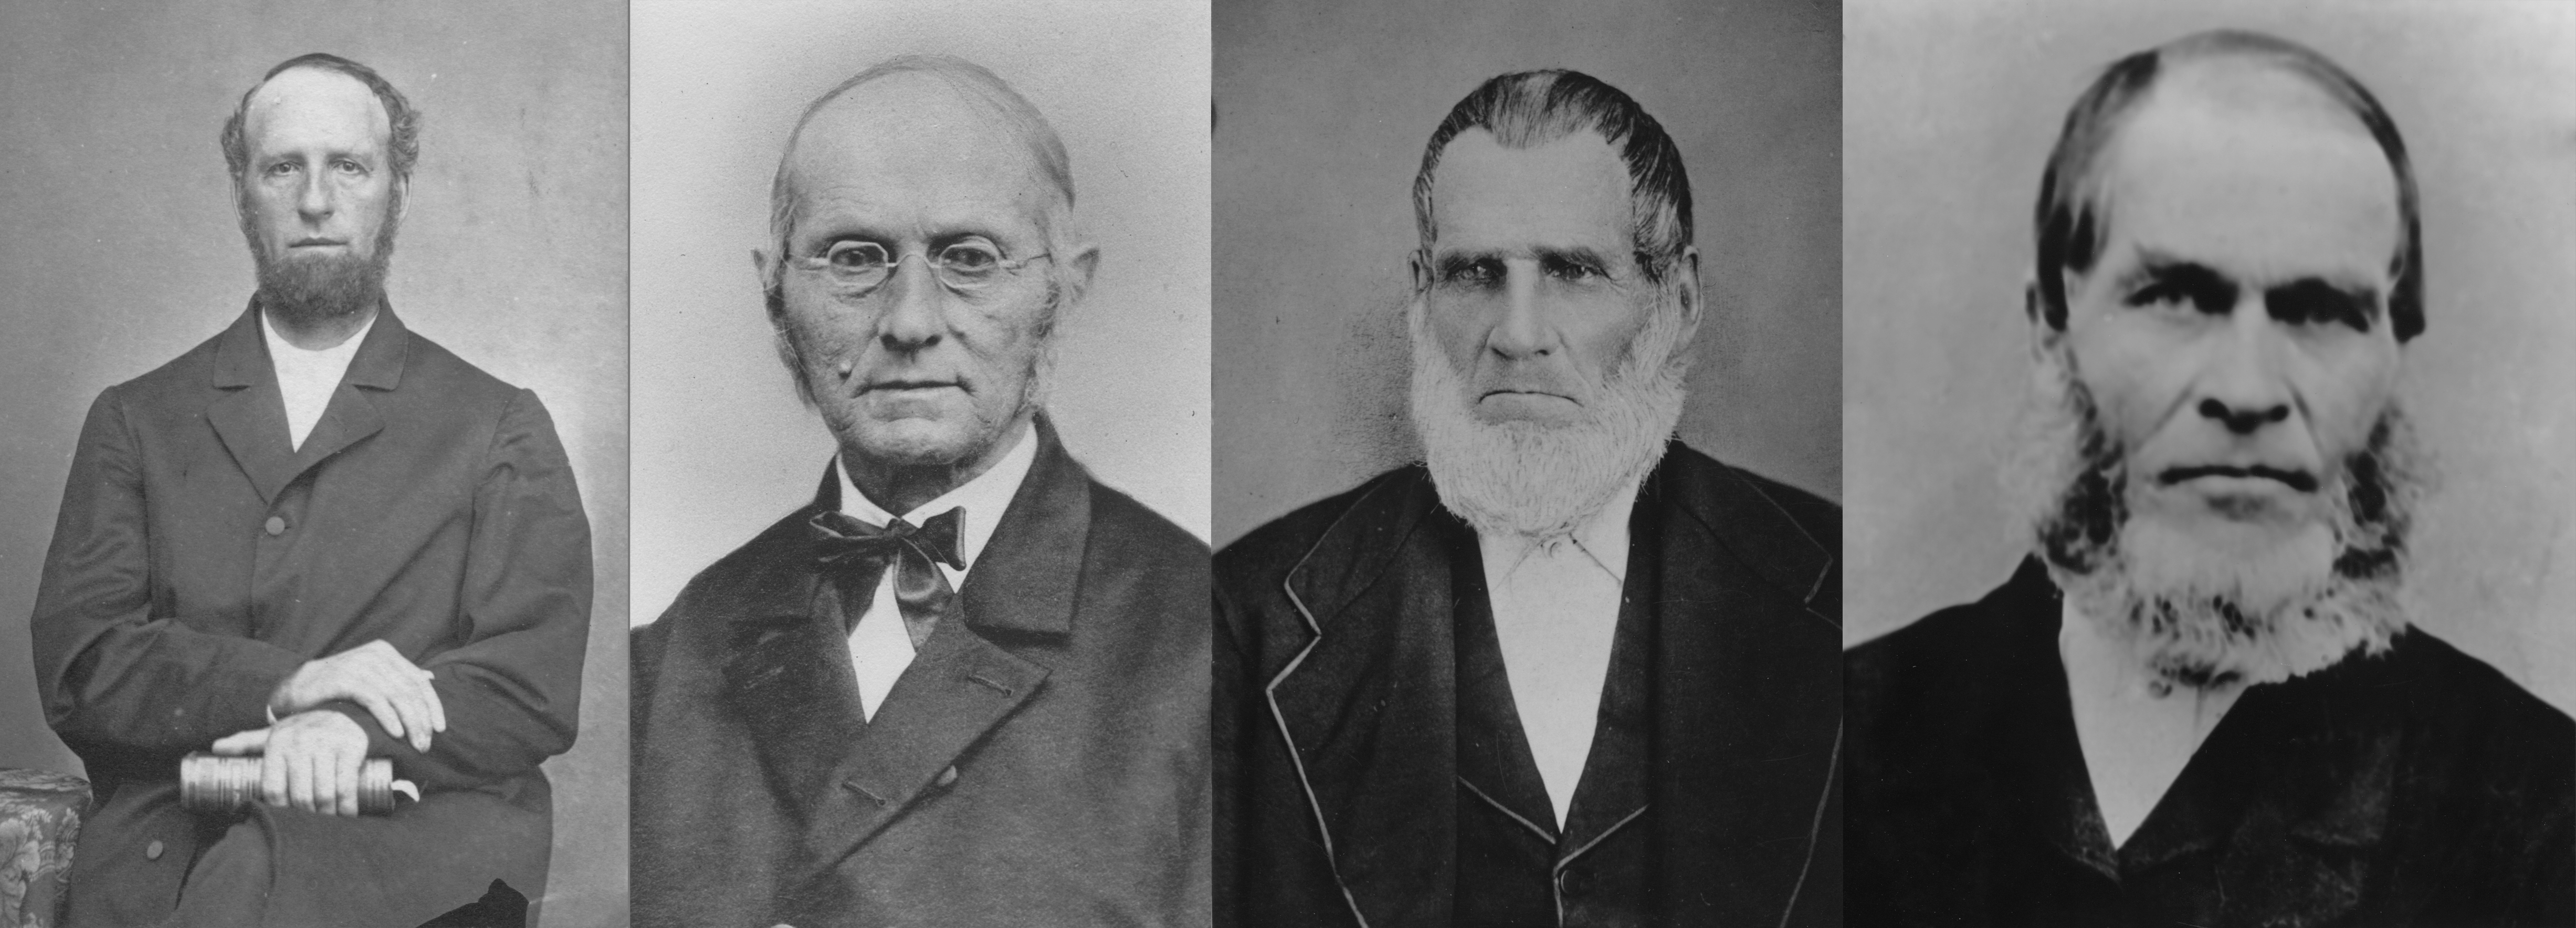
\includegraphics[width=1\linewidth]{images/james-white-joseph-bates-stephen-pierce-hiram-edson.jpg}
    \caption*{James White, Joseph Bates, Stephen Pierce, Hiram Edson}
    \label{fig:pioneers}
\end{figure}


\begin{figure}
    \centering
    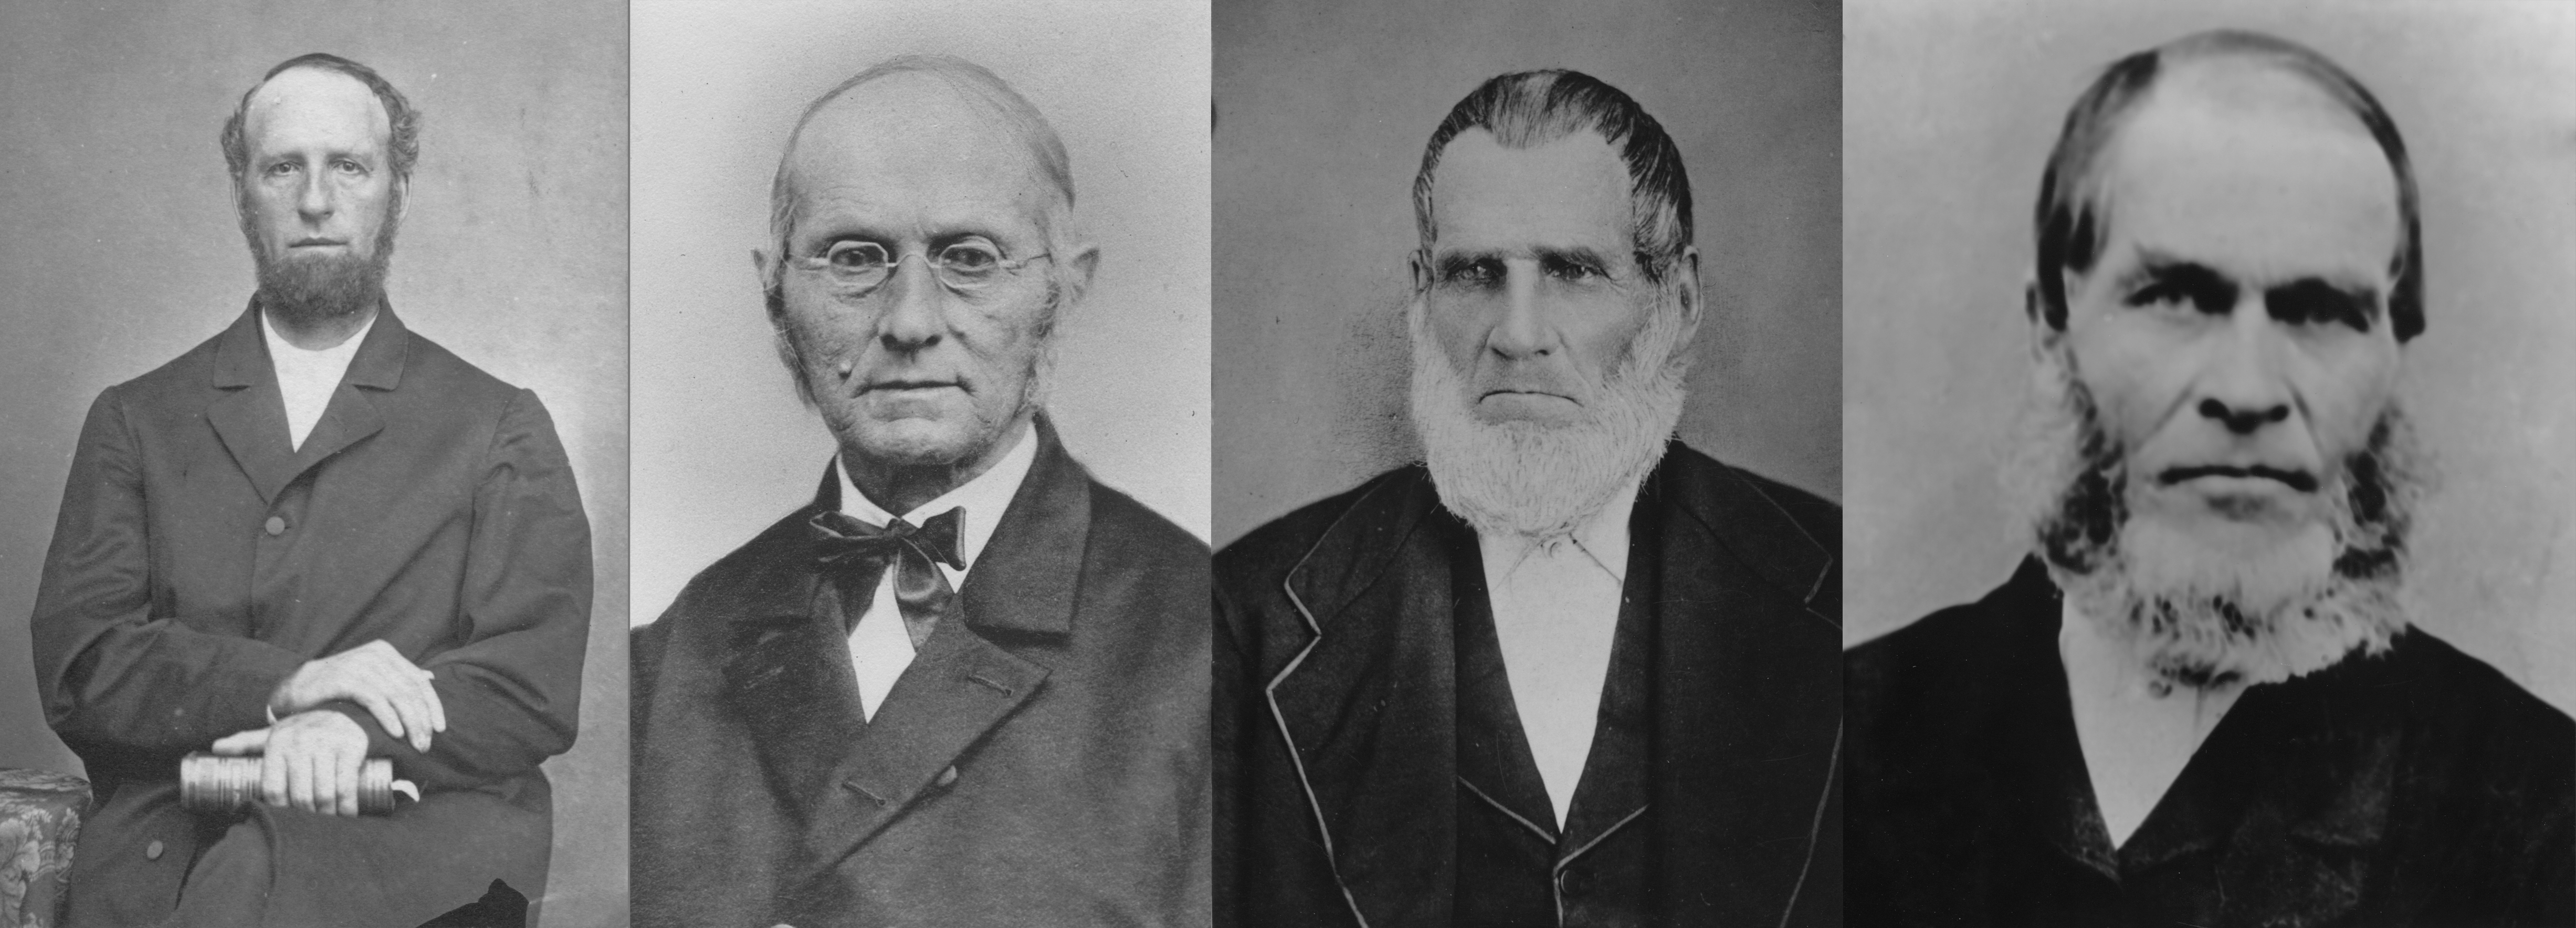
\includegraphics[width=1\linewidth]{images/james-white-joseph-bates-stephen-pierce-hiram-edson.jpg}
    \caption*{James White, Joseph Bates, Stephen Pierce, Hiram Edson}
    \label{fig:pioneers}
\end{figure}


\egwnogap{During this whole time I could not understand the reasoning of the brethren. My mind was locked, as it were, and I could not comprehend the meaning of the scriptures we were studying. This was one of the greatest sorrows of my life. \textbf{I was in this condition of mind until all \underline{the principal points of our faith} were made clear to our minds, in harmony with the word of God}. The brethren knew that when not in vision, I could not understand these matters, and they accepted as light direct from heaven the revelations given.}[SpTB02 57.1; 1904][https://egwwritings.org/read?panels=p417.291]


\egwnogap{Durante todo ese tiempo, no podía entender el razonamiento de los hermanos. Mi mente estaba cerrada, por así decirlo, y no podía comprender el significado de las Escrituras que estábamos estudiando. Este fue uno de los mayores dolores de mi vida. \textbf{Quedaba en esta condición mental hasta que se aclaraban en nuestras mentes todos \underline{los principales puntos de nuestra fe}, en armonía con la Palabra de Dios}. Los hermanos sabían que cuando yo no estaba en visión, no podía entender esos asuntos, y aceptaban como luz enviada del cielo las revelaciones dadas.}[SpTB02 57.1; 1904][https://egwwritings.org/read?panels=p417.291]


\egwnogap{For two or three years my mind continued to be locked to an understanding of the Scriptures. In the course of our labors, my husband and I visited Father Andrews, who was suffering intensely with inflammatory rheumatism. We prayed for him. I laid my hands on his head, and said, ‘Father Andrews, the Lord Jesus maketh thee whole.’ He was healed instantly. He got up, and walked about the room, praising God, and saying, ‘I never saw it on this wise before. Angels of God are in this room.’ The glory of the Lord was revealed. Light seemed to shine all through the house, and an angel’s hand was laid upon my head. From that time to this I have been able to understand the word of God.}[SpTB02 57.2; 1904][https://egwwritings.org/read?panels=p417.292]


\egwnogap{Durante dos o tres años, mi mente continuó cerrada a la comprensión de las Escrituras. En el curso de nuestras tareas, mi esposo y yo visitamos al padre Andrews, que estaba sufriendo intensamente de reumatismo inflamatorio. Oramos por él. Puse mis manos sobre su cabeza y dije: “Padre Andrews, el Señor Jesús te sana”. Fue sanado instantáneamente. Se levantó y caminó por la habitación alabando a Dios y diciendo: “Nunca antes vi cosa semejante. Ángeles de Dios están en esta habitación”. La gloria del Señor fue revelada. La luz parecía brillar por toda la casa y la mano de un ángel reposó sobre mi cabeza. Desde ese momento hasta ahora, he podido entender la Palabra de Dios.}[SpTB02 57.2; 1904][https://egwwritings.org/read?panels=p417.292]


\egwnogap{\textbf{What influence is it that would lead men at this stage of our history to work in an underhanded, powerful way \underline{to tear down the foundation of our faith},—the foundation that was laid at the beginning of our work by prayerful study of the word and by revelation? Upon \underline{this foundation} we have been building for \underline{the past fifty years}. Do you wonder that when I see the beginning of a work that would \underline{remove some of the pillars of our faith}, I have something to say? I must obey the command, ‘Meet it!’}}[SpTB02 58.1; 1904][https://egwwritings.org/read?panels=p417.295]


\egwnogap{\textbf{¿Qué influencia es la que induciría a los hombres en esta etapa de nuestra historia para proceder en una forma solapada y poderosa \underline{para derribar el fundamento de nuestra fe},—el fundamento que fue colocado al principio de nuestra obra mediante estudio de la Palabra acompañado de oración y mediante revelación? Sobre \underline{este fundamento} hemos estado construyendo durante \underline{los últimos cincuenta años}. ¿Os sorprende que cuando veo el comienzo de una obra que \underline{desplazaría algunas de las columnas de nuestra fe}, tenga yo algo que decir? Debo obedecer la orden: ‘¡Hazle frente!’}}[SpTB02 58.1; 1904][https://egwwritings.org/read?panels=p417.295]


\egwnogap{I have the tenderest feelings toward Dr. Kellogg. For many years I have tried to hold fast to him. God’s word to me has always been, ‘You can help him.’ Sometimes I am awakened in the night, and, rising, I walk the room, praying: ‘O Lord, hold Dr. Kellogg fast. Do not let him go. Keep him steadfast. Anoint his eyes with the heavenly eyesalve, that he may see all things clearly.’ Night after night I have lain awake, studying how I could help him. Earnestly and often I have prayed that the Lord may not permit him to turn away from sanctifying truth. This is the burden that weighs me down,—the desire that he shall be kept from making mistakes that would hurt his soul and \textbf{injure the cause of present truth}. But for some time his actions have revealed that a strange spirit is controlling him. The Lord will take this matter in His own hands. I must bear the messages of warning that God gives me to bear, and then leave with the Lord the results. \textbf{I must now present the matter in all its bearings; for the people of God must not be despoiled}.}[SpTB02 58.2; 1904][https://egwwritings.org/read?panels=p417.296]


\egwnogap{Tengo los más tiernos sentimientos hacia el Dr. Kellogg. Durante muchos años he tratado de aferrarme a él. La palabra de Dios para mí siempre ha sido: “Puedes ayudarlo”. A veces me despierto por la noche y, al levantarme, camino por la habitación, rezando: “Oh, Señor, sujeta al Dr. Kellogg. No lo dejes ir. Manténlo firme. Unge sus ojos con el colirio celestial, para que pueda ver todas las cosas con claridad”. Noche tras noche he permanecido despierta, estudiando cómo podría ayudarle. He orado con frecuencia y sinceramente para que el Señor no le permita apartarse de la verdad santificadora. Esta es la carga que me pesa, el deseo de que se le impida cometer errores que puedan dañar su alma y \textbf{perjudicar la causa de la verdad presente}. Pero durante algún tiempo sus acciones han revelado que un espíritu extraño lo está controlando. El Señor tomará este asunto en sus propias manos. Debo llevar los mensajes de advertencia que Dios me da para llevar, y luego dejar con el Señor los resultados. \textbf{Ahora debo presentar el asunto en todos sus aspectos; porque el pueblo de Dios no debe ser despojado}.}[SpTB02 58.2; 1904][https://egwwritings.org/read?panels=p417.296]


\egwnogap{\textbf{We are God’s commandment-keeping people. For the past fifty years every phase of heresy has been brought to bear upon us, to becloud our minds regarding the teaching of the word},\textbf{—especially concerning the ministration of Christ in the heavenly sanctuary, and the message of heaven for these last days, as given by the angels of the fourteenth chapter of Revelation}. \textbf{Messages of every order and kind have been urged upon Seventh-day Adventists, to take the place of the truth which, \underline{point by point}, has been sought out by prayerful study, and testified to by the miracle-working power of the Lord}. \textbf{But \underline{the way-marks} \underline{which have made us what we are}, \underline{are to be preserved}, and they \underline{will be preserved}, as God has signified through His word and the testimony of His Spirit}. \textbf{He calls upon us to \underline{hold firmly}, with the grip of faith, to \underline{the fundamental principles} that are \underline{based upon unquestionable authority}}.}[SpTB02 59.1; 1904][https://egwwritings.org/read?panels=p417.299]


\egwnogap{\textbf{Somos el pueblo que guarda los mandamientos de Dios. Durante los últimos cincuenta años toda suerte de herejías han sido presentadas para dominarnos, para nublar nuestras mentes acerca de la enseñanza de la Palabra},\textbf{—especialmente acerca de la ministración de Cristo en el santuario celestial, y el mensaje del cielo para estos últimos días, como es dado por los ángeles del capítulo 14 del Apocalipsis}. \textbf{Mensajes de toda especie han sido presentados a los adventistas del séptimo día, para ocupar el lugar de la verdad que, \underline{punto por punto}, ha sido descubierta mediante estudio con oración, y testificada mediante el poder del Señor que obra milagros}. \textbf{Pero \underline{los hitos} \underline{que nos han hecho lo que somos}, \underline{han de ser preservados}, y \underline{serán preservados}, como Dios lo ha manifestado mediante su Palabra y el testimonio de su Espíritu}. \textbf{Él nos insta a \underline{aferrarnos firmemente}, con el vigor de la fe, a \underline{los principios fundamentales} que están \underline{basados sobre una autoridad incuestionable}}.}[SpTB02 59.1; 1904][https://egwwritings.org/read?panels=p417.299]


There was a necessity to warn the church of the development of the enemy to uproot the foundation of our faith. There was a necessity to remind the church of what constitutes the true foundation of Seventh-day Adventist faith. It seems that Seventh-day Adventists, at that time, were forgetting \egwinline{the way the Lord has led us, and His teaching in our past history.}[LS 196.2; 1915][https://egwwritings.org/read?panels=p41.1083]


Había una necesidad de advertir a la iglesia del desarrollo del enemigo para desarraigar el fundamento de nuestra fe. Había una necesidad de recordar a la iglesia lo que constituye el verdadero fundamento de la fe adventista del séptimo día. Parece que los adventistas del séptimo día, en ese momento, estaban olvidando \egwinline{la manera en que el Señor nos ha conducido, y Su enseñanza en nuestra historia pasada.}[LS 196.2; 1915][https://egwwritings.org/read?panels=p41.1083]


\egw{What influence is it that would lead men at this stage of our history to work in an underhanded, powerful way \textbf{to tear down the foundation of our faith},—the foundation that was laid \textbf{at the beginning of our work} by prayerful study of the word and by revelation? Upon \textbf{this foundation} we have been building for \textbf{the past fifty years}. Do you wonder that when I see the beginning of a work that would \textbf{remove some of the pillars of our faith}, I have something to say? I must obey the command, ‘\textbf{Meet it}!’}[SpTB02 58.1; 1904][https://egwwritings.org/read?panels=p417.295]


\egw{¿Qué influencia es la que induciría a los hombres en esta etapa de nuestra historia para proceder en una forma solapada y poderosa \textbf{para derribar el fundamento de nuestra fe},—el fundamento que fue colocado \textbf{al principio de nuestra obra} mediante estudio de la Palabra acompañado de oración y mediante revelación? Sobre \textbf{este fundamento} hemos estado construyendo durante \textbf{los últimos cincuenta años}. ¿Os sorprende que cuando veo el comienzo de una obra que \textbf{desplazaría algunas de las columnas de nuestra fe}, tenga yo algo que decir? Debo obedecer la orden: ‘\textbf{¡Hazle frente}!’}[SpTB02 58.1; 1904][https://egwwritings.org/read?panels=p417.295]


What was it that Sister White was commanded to meet?


¿Qué fue lo que se le ordenó a la hermana White que enfrentara?


\egwinline{About the time that ‘Living Temple’ was published} in the night season she received \egwinline{representations indicating that some danger was approaching,} and that she must \egwinline{prepare for it by writing out the things God has revealed} to her \egwinline{\textbf{regarding the foundation principles of our faith}.}


\egwinline{Por el tiempo cuando se publicó ‘Living Temple’} en la temporada nocturna ella recibió \egwinline{representaciones que indicaban que algún peligro se avecinaba,} y que debía \egwinline{prepararse para él poniendo por escrito las cosas que Dios me había revelado} a ella \egwinline{\textbf{acerca de los principios fundamentales de nuestra fe}.}


She was \egwinline{instructed by the heavenly messenger that some of the reasoning in the book, ‘Living Temple’, is unsound and that \textbf{this reasoning would lead astray} the minds of those who are not thoroughly established on \textbf{the foundation principles} of present truth.}


Ella fue \egwinline{instruida por el mensajero celestial de que parte del razonamiento del libro, ‘Living Temple’, es malsano y que \textbf{este razonamiento descarriaría} las mentes de aquellos que no están plenamente establecidos en \textbf{los principios fundamentales} de la verdad presente.}


So, what was the actual problem with the book, “Living Temple”?


Entonces, ¿cuál era el problema real con el libro “Living Temple”?


If you are a scholar, or an Adventist historian, or a theologian, or just a student of theology, before you give a straight answer and say that the problem was pantheism, we would like to point you back to the text. Sister White clearly addressed the core issue of the problem stating that the “Living Temple,” \egwinline{introduces that which is naught but speculation in \textbf{regard to the personality of God and where His presence is}.}


Si usted es un académico, o un historiador adventista, o un teólogo, o simplemente un estudiante de teología, antes de dar una respuesta directa y decir que el problema era el panteísmo, nos gustaría señalarle de nuevo el texto. La hermana White abordó claramente la cuestión central del problema afirmando que el “Living Temple”, \egwinline{introduce aquello que no es nada sino especulación en \textbf{cuanto a la personalidad de Dios y dónde está su presencia}.}


We do not deny the pantheistic problem of the book, but we want to divert attention from Kellogg’s error to the light God has given. There are two ways to approach Kellogg’s crisis. One is by addressing the pantheism, and another is to address \egwinline{\textbf{the personality of God} and \textbf{where His presence is}}. One way is to study the error, and the other way is to study the Truth. One way is to dissect the darkness and the other way is to drink from the fountain of the Truth. We choose the latter, and for this reason this book is set apart from hundreds of other books written on Kellogg’s crisis. The subject of this book is not pantheism, or any other error, but the truth and what God has revealed about His personality and where His presence is. This was the real issue of Kellogg’s publication.


No negamos el problema panteísta del libro, pero queremos desviar la atención del error de Kellogg hacia la luz que Dios ha dado. Hay dos maneras de abordar la crisis de Kellogg. Una es abordar el panteísmo, y otra es abordar \egwinline{\textbf{la personalidad de Dios} y \textbf{dónde está su presencia}}. Una manera es estudiar el error, y la otra manera es estudiar la Verdad. Una forma es diseccionar la oscuridad y la otra es beber de la fuente de la Verdad. Nosotros elegimos esta última, y por esta razón este libro se distingue de los cientos de otros libros escritos sobre la crisis de Kellogg. El tema de este libro no es el panteísmo, ni ningún otro error, sino la verdad y lo que Dios ha revelado sobre su personalidad y dónde está su presencia. Este fue el verdadero tema de la publicación de Kellogg.


We believe it is a great danger to study and dissect the error because error leads to deception. The problem with deception is that we could be deceived obviously not knowing we are deceived! We firmly believe that Ellen White was the prophet of God and that she was receiving the Light from God \bible{who is light and in Him is no darkness at all}[1 John 1:5]. Therefore, we do not expect Sister White to explain the error in the book, “Living Temple”. Many were coming to her, asking her \egwinline{to explain the positions taken in ‘Living Temple.’} She replied, \egwinline{They are unexplainable}. Her objective was not to dissect the error but to shine the Truth on the \emcap{personality of God} and where His presence is. Thus, she was pointing back to the truths God founded the Seventh-day Adventist Church on. These truths have been constituting the foundation of our faith. These truths have been given to us in our early days. By diverting our attention from the personality of God to pantheism, we are losing an opportunity to remember \egwinline{\textbf{the way the Lord has led us}, and \textbf{His teaching} in our \textbf{past history}}. In this light, we express our concern over the Kellogg crisis and its pantheistic approach, because \egwinline{the track of truth lies close beside the track of error, and both tracks may seem to be one}; the solution to that is to be \egwinline{thoroughly established on \textbf{the foundation principles} of present truth}. Elsewhere, Sister White strongly established this principle.


Creemos que es un gran peligro estudiar y diseccionar el error porque el error lleva al engaño. El problema con el engaño es que podemos ser engañados obviamente sin saber que estamos engañados. Creemos firmemente que Ellen White era la profeta de Dios y que estaba recibiendo la Luz de Dios \bible{quien es luz, y no hay ningunas tinieblas en él}[1 Juan 1:5]. Por lo tanto, no esperamos que la hermana White explique el error en el libro “Living Temple”. Muchos venían a ella, pidiéndole \egwinline{que explicara las posiciones tomadas en ‘Living Temple’.} Ella respondía, \egwinline{Son inexplicables}. Su objetivo no era diseccionar el error, sino hacer brillar la Verdad sobre la \emcap{personalidad de Dios} y dónde está Su presencia. Así, ella estaba señalando las verdades sobre las que Dios fundó la Iglesia Adventista del Séptimo Día. Estas verdades han constituido el fundamento de nuestra fe. Estas verdades nos han sido dadas en nuestros primeros días. Al desviar nuestra atención de la personalidad de Dios hacia el panteísmo, estamos perdiendo la oportunidad de recordar \egwinline{\textbf{la manera en que el Señor nos ha conducido}, y \textbf{Su enseñanza} en nuestra \textbf{historia pasada}}. A la luz de esto, expresamos nuestra preocupación por la crisis de Kellogg y su enfoque panteísta, porque \egwinline{el sendero de la verdad se halla al lado y cerca del sendero del error, y ambas sendas pueden parecer ser una}; la solución a eso es estar \egwinline{plenamente establecidos en \textbf{los principios fundamentales} de la verdad presente}. En otro lugar, la hermana White estableció firmemente este principio.


\egw{Satan is by no means asleep; he is wide-awake and is playing the game of life for the souls of the people of God. He will come to them with flattery of all kinds, in the hope of leading them to swerve from their allegiance. \textbf{He desires to call their attention from the real issues to false theories}.}[Ms132-1903.42; 1904][https://egwwritings.org/read?panels=p9056.56]


\egw{Satanás no está de ninguna manera dormido; está bien despierto y está jugando el juego de la vida por las almas del pueblo de Dios. Vendrá a ellos con halagos de todo tipo, con la esperanza de inducirlos a desviarse de su lealtad. \textbf{Desea llamar su atención desde los verdaderos problemas hacia las falsas teorías}.}[Ms132-1903.42; 1904][https://egwwritings.org/read?panels=p9056.56]


So, let us focus our attention on the real issue instead of the false theories.


Por lo tanto, enfoquemos nuestra atención en la verdadera cuestión en lugar de las falsas teorías.


% The Foundation of our Faith

\begin{titledpoem}
    \stanza{
        Pillars of truth, laid with care, \\
        By pioneers who sought in prayer. \\
        Principles firm, the Lord's design, \\
        A platform strong, for all time.
    }

    \stanza{
        Beware the subtle shifts that call, \\
        To change what should not change at all. \\
        Our identity, in these we find, \\
        God's revelations to mankind.
    }

    \stanza{
        Stand fast upon this solid ground, \\
        Where wisdom and God's light abound. \\
        Defend these truths with all your might, \\
        For in them shines eternal light.
    }
\end{titledpoem}


% \chapter{The Foundation of Our Faith}

\egw{\textbf{The Lord will put new, vital force into His work} as human agencies obey the command to go forth and proclaim the truth. \textbf{He who declared that His truth would shine forever will proclaim this truth through faithful messengers, who will give the trumpet a certain sound}. \textbf{The truth will be criticized, scorned, and derided; but the \underline{closer} it is examined and tested, \underline{the brighter it will shine}}.}[SpTB02 51.1; 1904][https://egwwritings.org/read?panels=p417.260]

\egwnogap{\textbf{As a people, we are to \underline{stand firm on the platform of eternal truth} that has withstood test and trial. We are to \underline{hold to the sure pillars of our faith}. The \underline{principles of truth} that God has revealed to us \underline{are our only true foundation}. They have made us what we are. The lapse of time has not lessened their value. \underline{It is the constant effort of the enemy to remove these truths from their setting}, and to put in their place \underline{spurious theories}. He \underline{will bring in} everything that he possibly can to carry out his deceptive designs. But the Lord will raise up men of keen perception, who will give these truths their proper place in the plan of God.}}[SpTB02 51.2; 1904][https://egwwritings.org/read?panels=p417.261]

\egwnogap{\textbf{I have been instructed by the heavenly messenger that some of the reasoning in the book, ‘Living Temple,’ is unsound and that \underline{this reasoning would lead astray} the minds of those who are not thoroughly established on \underline{the foundation principles} of present truth. It introduces that which is naught but speculation in \underline{regard to the personality of God and where His presence is}}. No one on this earth has a right to speculate on this question. \textbf{The more fanciful theories are discussed, the less men will know of God and of the truth that sanctifies the soul}.}[SpTB02 51.3; 1904][https://egwwritings.org/read?panels=p417.262]

\egwnogap{One and another come to me, asking me \textbf{to explain the positions taken in ‘Living Temple.’} I reply, ‘\textbf{They are unexplainable}.’ \textbf{The sentiments expressed do not give a true knowledge of God}. All through the book are passages of scripture. These scriptures are brought in in such a way that error is made to appear as truth. \textbf{Erroneous theories are presented in so pleasing a way that unless care is taken, many will be misled}.}[SpTB02 52.1; 1904][https://egwwritings.org/read?panels=p417.265]

\egwnogap{\textbf{We need not the mysticism that is in this book}. Those who entertain these sophistries will soon find themselves in a position where the enemy can talk with them, and lead them away from God. It is represented to me that the writer of this book is on a false track. \textbf{He has lost sight of the distinguishing truths for \underline{this time}}. He knows not whither his steps are tending. \textbf{\underline{The track of truth lies close beside the track of error}, and both tracks may seem to be one to minds which are not worked by the Holy Spirit, and which, therefore, are not quick to discern the difference between truth and error}.}[SpTB02 52.2; 1904][https://egwwritings.org/read?panels=p417.266]

\egwnogap{\textbf{About the time that ‘Living Temple’ was published, there passed before me in the night season, \underline{representations indicating that some danger was approaching}, and that I must prepare for it by \underline{writing out the things} God has revealed to me \underline{regarding the foundation principles of our faith}}.}[SpTB02 52.3; 1904][https://egwwritings.org/read?panels=p417.267]

\egwnogap{A copy of ‘Living Temple’ was sent me, but it remained in my library, unread. From the light given me by the Lord, \textbf{I knew that some of the sentiments advocated in the book, did not bear the indorsement of God}, \textbf{and that they were \underline{a snare that the enemy had prepared for the last days}}. I thought that this would surely be discerned, and that it would not be necessary for me to say anything about it.}[SpTB02 52.4; 1904][https://egwwritings.org/read?panels=p417.268]

\egwnogap{In the controversy that arose among our brethren \textbf{regarding the teachings of this book}, those in favor of giving it a wide circulation declared: ‘\textbf{It contains the very sentiments that Sister White has been teaching}.’ This assertion struck right to my heart. I felt heart-broken; for \textbf{I knew that this representation of the matter \underline{was not true}}.}[SpTB02 53.1; 1904][https://egwwritings.org/read?panels=p417.270]

\egwnogap{Finally my son said to me, ‘Mother, you ought to read at least some parts of the book, that you may see whether they are in harmony with the light that God has given you.’ He sat down beside me, and together \textbf{we read the preface, and most of the first chapter, and also paragraphs in other chapters}. As we read, I recognized the very sentiments against which I had been bidden to speak in warning \textbf{during \underline{the early days} of my public labors}. When I first left the State of Maine, it was to go through Vermont and Massachusetts, to bear a testimony against these sentiments. \textbf{‘Living Temple’ contains the alpha of these theories. I knew that the \underline{omega would follow in a little while}; and I trembled for our people}. \textbf{I knew that I must warn our brethren and sisters not to enter into controversy \underline{over the presence and personality of God}}. \textbf{The statements made in ‘Living Temple’ \underline{in regard to this point are incorrect}}. The scripture used to substantiate the doctrine there set forth, is scripture misapplied.}[SpTB02 53.2; 1904][https://egwwritings.org/read?panels=p417.271]

\egwnogap{\textbf{I am compelled to speak in denial of the claim that the teachings of ‘Living Temple’ can be sustained by statements from my writings}. \textbf{There may be in this book expressions and sentiments that are in harmony with my writings}. \textbf{And there may be in my writings many statements which, taken from their connection, and interpreted according to the mind of the writer of ‘Living Temple,’ would seem to be in harmony with the teachings of this book.} This may give apparent support to the assertion that the sentiments in ‘Living Temple’ are in harmony with my writings. \textbf{But God forbid that this sentiment should prevail}.}[SpTB02 53.3; 1904][https://egwwritings.org/read?panels=p417.272]

\egwnogap{\textbf{Few can discern the result of entertaining the sophistries advocated by some at this time}. \textbf{But the Lord has lifted the curtain, and has \underline{shown me the result that would follow}}. \textbf{The spiritualistic theories \underline{regarding the personality of God}, followed to their logical conclusion, sweep away the whole Christian economy}. \textbf{They estimate as nothing the light that Christ came from heaven to give John to give to His people. They teach that the scenes just before us are not of sufficient importance to be given special attention. They make of no effect the truth of heavenly origin, \underline{and rob the people of God of their past experience}, giving them instead a false science}.}[SpTB02 54.1; 1904][https://egwwritings.org/read?panels=p417.275]

\egwnogap{\textbf{In a vision} of the night I was shown distinctly that \textbf{these sentiments} have been looked upon by some as \textbf{the grand truths} \textbf{that are to be \underline{brought in}} and made prominent at the present time. \textbf{I was shown \underline{a platform}, braced by \underline{solid timbers},—the truths of the Word of God}. \textbf{Some one high in responsibility in the medical work was directing this man and that man to loosen the timbers supporting this platform}. Then I heard a voice saying, ‘Where are the watchmen that ought to be standing on the walls of Zion? Are they asleep? \textbf{\underline{This foundation was built by the Masterworker}, and \underline{will} stand storm and tempest. Will they permit this man to \underline{present doctrines} \underline{that deny the past experience} of the people of God? The time has come to take decided action}.’}[SpTB02 54.2; 1904][https://egwwritings.org/read?panels=p417.276]

\egwnogap{\textbf{The enemy of souls has sought to \underline{bring in} the supposition that \underline{a great reformation} was to take place among Seventh-day Adventists, and that \underline{this reformation} would \underline{consist in giving up the doctrines which stand as the pillars of our faith,} and engaging in a process of reorganization}. \textbf{Were this reformation to take place, \underline{what would result}?} \textbf{\underline{The principles of truth} that God in His wisdom has given to the remnant church, \underline{would be discarded}}. \textbf{Our religion would be changed}. \textbf{\underline{The fundamental principles} that have sustained the work for the last fifty years \underline{would be accounted as error}}. \textbf{A new organization would be established}. \textbf{Books of a new order would be written}.\textbf{ A system of intellectual philosophy would be introduced}. The founders of this system would go into the cities, and do a wonderful work. The Sabbath, of course, would be lightly regarded, \textbf{as also the God who created it}. Nothing would be allowed to stand in the way of the new movement. \textbf{The leaders would teach that virtue is better than vice, but God being removed, they would place their dependence on human power, which, without God, is worthless}. \textbf{Their foundation would be built on the sand, and storm and tempest would sweep away the structure}.}[SpTB02 54.3; 1904][https://egwwritings.org/read?panels=p417.277]

\egwnogap{Who has authority to begin such a movement? \textbf{We have our Bibles}. \textbf{We have our experience, attested to by the miraculous working of the Holy Spirit}. \textbf{We have a truth that admits of no compromise}. \textbf{\underline{Shall we not repudiate everything that is not in harmony with this truth}}?}[SpTB02 55.1; 1904][https://egwwritings.org/read?panels=p417.280]

\egwnogap{I hesitated and delayed about the sending out of that which the Spirit of the Lord impelled me to write. \textbf{I did not want to be compelled to present the misleading influence of these sophistries. But in the providence of God, the errors that have been coming in must be met}.}[SpTB02 55.2; 1904][https://egwwritings.org/read?panels=p417.281]

\egwnogap{Shortly before \textbf{I sent out the testimonies regarding the \underline{efforts of the enemy to undermine the foundation of our faith} through the dissemination of \underline{seductive theories}}, I had read an incident about a ship in a fog meeting an iceberg. For several nights I slept but little. I seemed to be bowed down as a cart beneath sheaves. One night a scene was clearly presented before me. A vessel was upon the waters, in a heavy fog. Suddenly the lookout cried, ‘Iceberg just ahead!’ There, towering high above the ship, was a gigantic iceberg. An authoritative voice cried out, ‘Meet it!’ There was not a moment’s hesitation. It was a time for instant action. The engineer put on full steam, and the man at the wheel steered the ship straight into the iceberg. With a crash she struck the ice. There was a fearful shock, and the iceberg broke into many pieces, falling with a noise like thunder to the deck. The passengers were violently shaken by the force of the collision, but no lives were lost. The vessel was injured, but not beyond repair. She rebounded from the contact, trembling from stem to stern, like a living creature. Then she moved forward on her way.}[SpTB02 55.3; 1904][https://egwwritings.org/read?panels=p417.282]

\egwnogap{Well I knew the meaning of this representation. \textbf{I had my orders}. I had heard the words, like a voice from our Captain, ‘\textbf{Meet it}!’ I knew what my duty was, and that there was not a moment to lose. The time for decided action had come. \textbf{I must without delay obey the command, ‘Meet it!’}}[SpTB02 56.1; 1904][https://egwwritings.org/read?panels=p417.285]

\egwnogap{That night I was up at one o’clock, writing as fast as my hand could pass over the paper. For the next few days I worked early and late, \textbf{preparing for our people the instruction given me \underline{regarding the errors} that were \underline{coming in} among us}.}[SpTB02 56.2; 1904][https://egwwritings.org/read?panels=p417.286]

\egwnogap{\textbf{I have been hoping that there would be a thorough reformation, and that \underline{the principles} for which we fought \underline{in the early days}, and which were brought out in the power of the Holy Spirit, \underline{would be maintained}}.}[SpTB02 56.3; 1904][https://egwwritings.org/read?panels=p417.287]

\egwnogap{\textbf{Many of our people do not realize \underline{how firmly} the foundation of our faith has been laid}. \textbf{My husband, Elder Joseph Bates, Father Pierce, Elder Edson, and others who were keen, noble, and true, were among those who, after the passing of the time in 1844, searched for the truth as for hidden treasure}. I met with them, and we studied and prayed earnestly. Often we remained together until late at night, and sometimes through the entire night, praying for light and studying the word. Again and again these brethren came together to study the Bible, in order that they might know its meaning, and be prepared to teach it with power. When they came to the point in their study where they said, ‘We can do nothing more,’ the Spirit of the Lord would come upon me, I would be taken off in vision, and a clear explanation of the passages we had been studying would be given me, with instruction as to how we were to labor and teach effectively. Thus light was given that helped us to understand the scriptures in regard to Christ, His mission, and His priesthood. \textbf{A line of truth extending from that time to the time when we shall enter the city of God, was made plain to me, and I gave to others the instruction that the Lord had given me}.}[SpTB02 56.4; 1904][https://egwwritings.org/read?panels=p417.288]

\egwnogap{During this whole time I could not understand the reasoning of the brethren. My mind was locked, as it were, and I could not comprehend the meaning of the scriptures we were studying. This was one of the greatest sorrows of my life. \textbf{I was in this condition of mind until all \underline{the principal points of our faith} were made clear to our minds, in harmony with the word of God}. The brethren knew that when not in vision, I could not understand these matters, and they accepted as light direct from heaven the revelations given.}[SpTB02 57.1; 1904][https://egwwritings.org/read?panels=p417.291]

\egwnogap{For two or three years my mind continued to be locked to an understanding of the Scriptures. In the course of our labors, my husband and I visited Father Andrews, who was suffering intensely with inflammatory rheumatism. We prayed for him. I laid my hands on his head, and said, ‘Father Andrews, the Lord Jesus maketh thee whole.’ He was healed instantly. He got up, and walked about the room, praising God, and saying, ‘I never saw it on this wise before. Angels of God are in this room.’ The glory of the Lord was revealed. Light seemed to shine all through the house, and an angel’s hand was laid upon my head. From that time to this I have been able to understand the word of God.}[SpTB02 57.2; 1904][https://egwwritings.org/read?panels=p417.292]

\egwnogap{\textbf{What influence is it that would lead men at this stage of our history to work in an underhanded, powerful way \underline{to tear down the foundation of our faith},—the foundation that was laid at the beginning of our work by prayerful study of the word and by revelation? Upon \underline{this foundation} we have been building for \underline{the past fifty years}. Do you wonder that when I see the beginning of a work that would \underline{remove some of the pillars of our faith}, I have something to say? I must obey the command, ‘Meet it!’}}[SpTB02 58.1; 1904][https://egwwritings.org/read?panels=p417.295]

\egwnogap{I have the tenderest feelings toward Dr. Kellogg. For many years I have tried to hold fast to him. God’s word to me has always been, ‘You can help him.’ Sometimes I am awakened in the night, and, rising, I walk the room, praying: ‘O Lord, hold Dr. Kellogg fast. Do not let him go. Keep him steadfast. Anoint his eyes with the heavenly eyesalve, that he may see all things clearly.’ Night after night I have lain awake, studying how I could help him. Earnestly and often I have prayed that the Lord may not permit him to turn away from sanctifying truth. This is the burden that weighs me down,—the desire that he shall be kept from making mistakes that would hurt his soul and \textbf{injure the cause of present truth}. But for some time his actions have revealed that a strange spirit is controlling him. The Lord will take this matter in His own hands. I must bear the messages of warning that God gives me to bear, and then leave with the Lord the results. \textbf{I must now present the matter in all its bearings; for the people of God must not be despoiled}.}[SpTB02 58.2; 1904][https://egwwritings.org/read?panels=p417.296]

\egwnogap{\textbf{We are God’s commandment-keeping people. For the past fifty years every phase of heresy has been brought to bear upon us, to becloud our minds regarding the teaching of the word},\textbf{—especially concerning the ministration of Christ in the heavenly sanctuary, and the message of heaven for these last days, as given by the angels of the fourteenth chapter of Revelation}. \textbf{Messages of every order and kind have been urged upon Seventh-day Adventists, to take the place of the truth which, \underline{point by point}, has been sought out by prayerful study, and testified to by the miracle-working power of the Lord}. \textbf{But \underline{the way-marks} \underline{which have made us what we are}, \underline{are to be preserved}, and they \underline{will be preserved}, as God has signified through His word and the testimony of His Spirit}. \textbf{He calls upon us to \underline{hold firmly}, with the grip of faith, to \underline{the fundamental principles} that are \underline{based upon unquestionable authority}}.}[SpTB02 59.1; 1904][https://egwwritings.org/read?panels=p417.299]

There was a necessity to warn the church of the development of the enemy to uproot the foundation of our faith. There was a necessity to remind the church of what constitutes the true foundation of Seventh-day Adventist faith. It seems that Seventh-day Adventists, at that time, were forgetting \egwinline{the way the Lord has led us, and His teaching in our past history.}[LS 196.2; 1915][https://egwwritings.org/read?panels=p41.1083]

\egw{What influence is it that would lead men at this stage of our history to work in an underhanded, powerful way \textbf{to tear down the foundation of our faith},—the foundation that was laid \textbf{at the beginning of our work} by prayerful study of the word and by revelation? Upon \textbf{this foundation} we have been building for \textbf{the past fifty years}. Do you wonder that when I see the beginning of a work that would \textbf{remove some of the pillars of our faith}, I have something to say? I must obey the command, ‘\textbf{Meet it}!’}[SpTB02 58.1; 1904][https://egwwritings.org/read?panels=p417.295]

What was it that Sister White was commanded to meet?

\egwinline{About the time that ‘Living Temple’ was published} in the night season she received \egwinline{representations indicating that some danger was approaching,} and that she must \egwinline{prepare for it by writing out the things God has revealed} to her \egwinline{\textbf{regarding the foundation principles of our faith}.}

She was \egwinline{instructed by the heavenly messenger that some of the reasoning in the book, ‘Living Temple’, is unsound and that \textbf{this reasoning would lead astray} the minds of those who are not thoroughly established on \textbf{the foundation principles} of present truth.}

So, what was the actual problem with the book, “Living Temple”?

If you are a scholar, or an Adventist historian, or a theologian, or just a student of theology, before you give a straight answer and say that the problem was pantheism, we would like to point you back to the text. Sister White clearly addressed the core issue of the problem stating that the “Living Temple,” \egwinline{introduces that which is naught but speculation in \textbf{regard to the personality of God and where His presence is}.}

We do not deny the pantheistic problem of the book, but we want to divert attention from Kellogg’s error to the light God has given. There are two ways to approach Kellogg’s crisis. One is by addressing the pantheism, and another is to address \egwinline{\textbf{the personality of God} and \textbf{where His presence is}}. One way is to study the error, and the other way is to study the Truth. One way is to dissect the darkness and the other way is to drink from the fountain of the Truth. We choose the latter, and for this reason this book is set apart from hundreds of other books written on Kellogg’s crisis. The subject of this book is not pantheism, or any other error, but the truth and what God has revealed about His personality and where His presence is. This was the real issue of Kellogg’s publication. 

We believe it is a great danger to study and dissect the error because error leads to deception. The problem with deception is that we could be deceived obviously not knowing we are deceived! We firmly believe that Ellen White was the prophet of God and that she was receiving the Light from God \bible{who is light and in Him is no darkness at all}[1 John 1:5]. Therefore, we do not expect Sister White to explain the error in the book, “Living Temple”. Many were coming to her, asking her \egwinline{to explain the positions taken in ‘Living Temple.’} She replied, \egwinline{They are unexplainable}. Her objective was not to dissect the error but to shine the Truth on the \emcap{personality of God} and where His presence is. Thus, she was pointing back to the truths God founded the Seventh-day Adventist Church on. These truths have been constituting the foundation of our faith. These truths have been given to us in our early days. By diverting our attention from the personality of God to pantheism, we are losing an opportunity to remember \egwinline{\textbf{the way the Lord has led us}, and \textbf{His teaching} in our \textbf{past history}}. In this light, we express our concern over the Kellogg crisis and its pantheistic approach, because \egwinline{the track of truth lies close beside the track of error, and both tracks may seem to be one}; the solution to that is to be \egwinline{thoroughly established on \textbf{the foundation principles} of present truth}. Elsewhere, Sister White strongly established this principle.

\egw{Satan is by no means asleep; he is wide-awake and is playing the game of life for the souls of the people of God. He will come to them with flattery of all kinds, in the hope of leading them to swerve from their allegiance. \textbf{He desires to call their attention from the real issues to false theories}.}[Ms132-1903.42; 1904][https://egwwritings.org/read?panels=p9056.56]

So, let us focus our attention on the real issue instead of the false theories. 

